\documentclass[a4paper,11pt]{article}
\input{/home/tof/Documents/Cozy/latex-include/preambule_doc.tex}
\input{/home/tof/Documents/Cozy/latex-include/preambule_commun.tex}
\newcommand{\showprof}{show them}  % comment this line if you don't want to see todo environment
\setlength{\fboxrule}{0.8pt}
\fancyhead[L]{\fbox{\Large{\textbf{RecTex 01}}}}
\fancyhead[C]{\textbf{Recherche textuelle}}
\newdate{madate}{10}{09}{2020}
%\fancyhead[R]{\displaydate{madate}} %\today
%\fancyhead[R]{Seconde - SNT}
%\fancyhead[R]{Première - NSI}
\fancyhead[R]{Terminale - NSI}
\fancyfoot[L]{\vspace{1mm}Christophe Viroulaud}
\AtEndDocument{\label{lastpage}}
\fancyfoot[C]{\textbf{Page \thepage/\pageref{lastpage}}}
\fancyfoot[R]{\includegraphics[width=2cm,align=t]{/home/tof/Documents/Cozy/latex-include/cc.png}}
\usepackage{tikz}

\begin{document}
\section{Problématique}
Rechercher les occurrences d'un mot dans un texte est une fonctionnalité intégrée dans tous les logiciels de traitements de texte. Si la tâche semble aisée dans un texte d'une seule page, nous pouvons nous interroger sur l'efficacité de la recherche d'un mot dans un livre entier.
%également dans EDI
\begin{center}
    \framebox{Comment effectuer une recherche textuelle efficace?}
\end{center}
\section{Approche naïve}
La première méthode à laquelle nous pouvons penser consiste à:
\begin{itemize}
    \item observer une \textbf{fenêtre} du texte,
    \item dans cette fenêtre, comparer chaque lettre du \textbf{motif} recherché au texte,
    \item décaler la fenêtre d'un cran dès qu'il n'y a pas de correspondance.
\end{itemize}
\begin{center}
    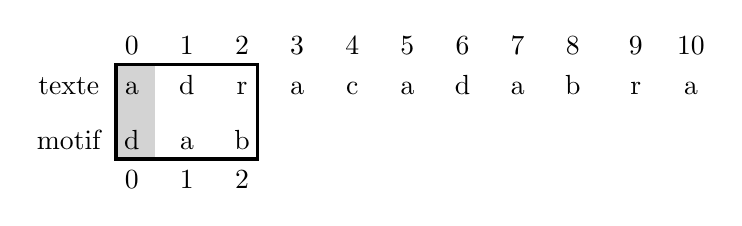
\begin{tikzpicture}
        \fill[LightGray] (1.9,0.5)--(2.4,0.5) -- (2.4,-0.7) -- (1.9,-0.7) -- cycle;
        \foreach \a/\b in {2.1/0,2.8/1,3.5/2,4.2/3,4.9/4,5.6/5,6.3/6,7/7,7.7/8,8.5/9,9.2/10}
            {\node[anchor=south] at (\a,0.5) {\b};}
        \node[anchor=south] at(1.3,0){texte};
        \foreach \a/\b in {2.1/a,2.8/d,3.5/r,4.2/a,4.9/c,5.6/a,6.3/d,7/a,7.7/b,8.5/r,9.2/a}
            {\node[anchor=south] at (\a,0) {\b};}

        \node[anchor=south] at(1.3,-0.7){motif};
        \foreach \a/\b in {2.1/d,2.8/a,3.5/b}
            {\node[anchor=south] at (\a,-0.7) {\b};}
        \foreach \a/\b in {2.1/0,2.8/1,3.5/2}
            {\node[anchor=south] at (\a,-1.2) {\b};}
        \draw[very thick] (1.9,0.5)--(3.7,0.5) -- (3.7,-0.7) -- (1.9,-0.7) -- cycle;
    \end{tikzpicture}
    \captionof{figure}{Première comparaison: pas de correspondance}
\end{center}
\begin{center}
    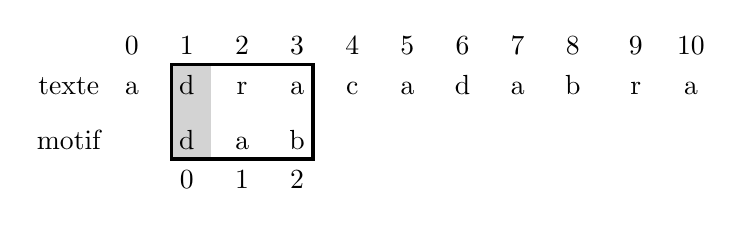
\begin{tikzpicture}
        \fill[LightGray] (2.6,0.5)--(3.1,0.5) -- (3.1,-0.7) -- (2.6,-0.7) -- cycle;
        \foreach \a/\b in {2.1/0,2.8/1,3.5/2,4.2/3,4.9/4,5.6/5,6.3/6,7/7,7.7/8,8.5/9,9.2/10}
            {\node[anchor=south] at (\a,0.5) {\b};}
        \node[anchor=south] at(1.3,0){texte};
        \foreach \a/\b in {2.1/a,2.8/d,3.5/r,4.2/a,4.9/c,5.6/a,6.3/d,7/a,7.7/b,8.5/r,9.2/a}
            {\node[anchor=south] at (\a,0) {\b};}

        \node[anchor=south] at(1.3,-0.7){motif};
        \foreach \a/\b in {2.8/d,3.5/a,4.2/b}
            {\node[anchor=south] at (\a,-0.7) {\b};}
        \foreach \a/\b in {2.8/0,3.5/1,4.2/2}
            {\node[anchor=south] at (\a,-1.2) {\b};}
        \draw[very thick] (2.6,0.5)--(4.4,0.5) -- (4.4,-0.7) -- (2.6,-0.7) -- cycle;
    \end{tikzpicture}
    \captionof{figure}{Première comparaison: correspondance}
\end{center}
\begin{center}
    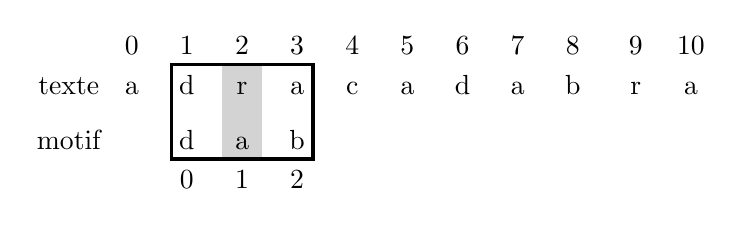
\begin{tikzpicture}
        \fill[LightGray] (3.25,0.5)--(3.75,0.5) -- (3.75,-0.7) -- (3.25,-0.7) -- cycle;
        \foreach \a/\b in {2.1/0,2.8/1,3.5/2,4.2/3,4.9/4,5.6/5,6.3/6,7/7,7.7/8,8.5/9,9.2/10}
            {\node[anchor=south] at (\a,0.5) {\b};}
        \node[anchor=south] at(1.3,0){texte};
        \foreach \a/\b in {2.1/a,2.8/d,3.5/r,4.2/a,4.9/c,5.6/a,6.3/d,7/a,7.7/b,8.5/r,9.2/a}
            {\node[anchor=south] at (\a,0) {\b};}

        \node[anchor=south] at(1.3,-0.7){motif};
        \foreach \a/\b in {2.8/d,3.5/a,4.2/b}
            {\node[anchor=south] at (\a,-0.7) {\b};}
        \foreach \a/\b in {2.8/0,3.5/1,4.2/2}
            {\node[anchor=south] at (\a,-1.2) {\b};}
        \draw[very thick] (2.6,0.5)--(4.4,0.5) -- (4.4,-0.7) -- (2.6,-0.7) -- cycle;
    \end{tikzpicture}
    \captionof{figure}{Deuxième comparaison: pas de correspondance}
\end{center}
\subsection{Implémentation}
\begin{activite}
    \begin{enumerate}
        \item Écrire la fonction \textbf{\texttt{recherche\_naive(texte: str, motif: str) $\rightarrow$ int}} qui renvoie la position du \emph{motif} dans le \emph{texte} ou -1 s'il n'est pas présent.
        \item Estimer la complexité temporelle de cet algorithme dans le pire des cas: le motif n'est pas présent dans le texte.
    \end{enumerate}
\end{activite}
\section{Approche plus efficace: Boyer-Moore}
%dvp en 1977
\subsection{Recherche à l'envers}
La première idée de cet algorithme est de commencer la recherche \textbf{en partant de la fin du motif}. 
% on parcourt toujours la chaîne de gauche à droite
\begin{center}
    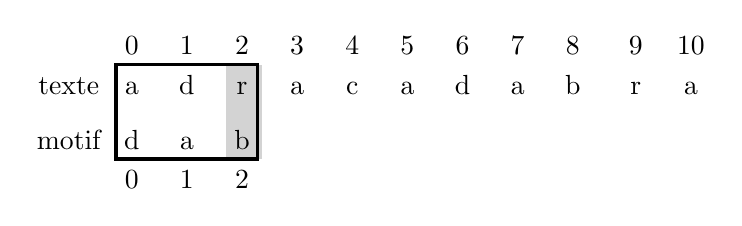
\begin{tikzpicture}
        \fill[LightGray] (3.3,0.5)--(3.75,0.5) -- (3.75,-0.7) -- (3.3,-0.7) -- cycle;
        \foreach \a/\b in {2.1/0,2.8/1,3.5/2,4.2/3,4.9/4,5.6/5,6.3/6,7/7,7.7/8,8.5/9,9.2/10}
            {\node[anchor=south] at (\a,0.5) {\b};}
        \node[anchor=south] at(1.3,0){texte};
        \foreach \a/\b in {2.1/a,2.8/d,3.5/r,4.2/a,4.9/c,5.6/a,6.3/d,7/a,7.7/b,8.5/r,9.2/a}
            {\node[anchor=south] at (\a,0) {\b};}

        \node[anchor=south] at(1.3,-0.7){motif};
        \foreach \a/\b in {2.1/d,2.8/a,3.5/b}
            {\node[anchor=south] at (\a,-0.7) {\b};}
        \foreach \a/\b in {2.1/0,2.8/1,3.5/2}
            {\node[anchor=south] at (\a,-1.2) {\b};}
        \draw[very thick] (1.9,0.5)--(3.7,0.5) -- (3.7,-0.7) -- (1.9,-0.7) -- cycle;
    \end{tikzpicture}
    \captionof{figure}{Première comparaison: pas de correspondance}
\end{center}
Pour l'instant cette approche ne semble par apporter d'amélioration par rapport à l'algorithme précédent.
\subsection{Décalages par sauts}

\subsection{Prétraitement du motif}
\end{document}